
% CS534 implementation assignment 1

\documentclass{article}

\usepackage{amsmath}
\usepackage{graphicx}
\usepackage{amsmath,amsthm,amssymb}
\usepackage[linesnumbered, ruled]{algorithm2e}
\SetKwRepeat{Do}{do}{while}%
\usepackage{titlesec}

\renewcommand{\labelenumi}{(\alph{enumi})}
\renewcommand{\vec}[1]{\mathbf{#1}}
%\algdef{SE}[DOWHILE]{Do}{doWhile}{\algorithmicdo}[1]{\algorithmicwhile\ #1}%

\titleformat{\section}
  {\normalfont\fontsize{12}{15}\bfseries}{\thesection}{1em}{}
\titleformat{\subsection}
  {\normalfont\fontsize{10}{12}\bfseries}{\thesubsection}{1em}{}

\begin{document}

\begin{center}
	{\huge CS-534 Machine Learning} \\ \vspace{2mm}
	{\Large Implementation Assignment 1} \\ \vspace{2mm} \hrule \vspace{3mm}
	{\normalsize Author 1 (\%) \hspace{6mm}  Author 2 (\%) \hspace{6mm}  Author 3 (\%)} 
\end{center}

\section{Introduction}

Given a set a $M$ training pairs $\{\vec{x}_i, y_i\}^M_{i=1}$, where $\vec{x}_i$ is a set of features $\{x_{ij}\}^N_{j=1}$ and $y_i$ is the corresponding target variable, we wish to find a set a parameters $\vec{w} = \{w_1, w_2, \dots ,w_n\}$ that minimizes the regularized Sum of Squared Error (SSE) objective

\begin{align*}
	J(\vec{w}) = \frac{1}{2}\sum^{m}_{i=1}(\vec{w}^\top\vec{x}_i - y_i)^2 + \lambda||\vec{w}||^2.
\end{align*}

Here, the regularization term $\lambda||\vec{w}||^2$ is used to counteract overfitting: a common artifact caused by high dimensional features. Overfitting is often manifest in large parameters, thus the regularization term to encourage small weights. $\lambda$ is a hyper-parameter that controls the influence of regularization on these weights and subsequent objective value and solution. This value is often not known and difficult to determine. The objective of this assignment is to implement the gradient descent algorithm (GDA) on a high dimensional training set and investigate the effect of the regularization parameter via cross-validation and validation using an independent dataset.

\subsection{Gradient descent algorithm}

To implement GDA, we first derive the gradient of the cost function $J(\vec{w})$. The gradient vector is of size $M$, the number of samples in the training set, and each element is equal to the partial derivative of the cost function $J(\vec{w})$ with respect to the parameters $\{w_i\}^N_{i=1}$. The chain rule gives

\begin{align}
	\nabla J(\vec{w}) = \left[\frac{\partial J}{\partial w_1}, \frac{\partial J}{\partial w_2},\dots, \frac{\partial J}{\partial w_n}\right]^\top .
\end{align}

Thus, the $k^{th}$ element of the gradient vector is 

\begin{align}
\frac{\partial J}{\partial w_k} = \sum^{m}_{i=1}(\vec{w}^\top\vec{x}_i - y_i)x_{ik} + 2\lambda\vec{w}.
\end{align}


This gives the following regularized gradient of the cost function $J(\vec{w})$:

\begin{align}
	\nabla J(\vec{w}) = \frac{1}{m} \sum^{m}_{i=1}(\vec{w}^\top\vec{x}_i - y_i)\vec{x}_i + 2\lambda\vec{w}.
\end{align}

Note that we have scaled the first term by the number of samples in the equation to represent the average gradient per weight. The gradient is now incorporated into the update rule for gradient descent. For a given training pair $\{\vec{x}_i, y_i\}$, the batch update rule is

\begin{align}
w_j =: w_j - \alpha\big((\vec{w}^\top \vec{x}_i - y_i)x_{ij} + 2\lambda w_j\big).
\end{align}

Equations 3 and 4 are used in a batch gradient descent algorithm where the parameters $\vec{w}$ are updated simultaneously across features until the norm of $\nabla J(\vec{w})$ converges at a small value $\epsilon$. To improve the speed of convergence we will also standardize the features by $s(\vec{x}) = \frac{\vec{x} - \bar{\vec{x}}}{\sigma}$.

\vspace{3mm}

\begin{algorithm}[H]
	\SetAlgoLined
	$\vec{w} = \vec{w}^{\vec{0}}$\;
	\Do{$|\nabla J(\vec{w})| \ge \epsilon$}{
		$\nabla J(\vec{w}) = \frac{1}{m} \sum^{m}_{i=1}(\vec{w}^\top\vec{x}_i - y_i)\vec{x}_i + 2\lambda\vec{w}$\;
		$\vec{w} =: \vec{w} - \alpha\nabla J(\vec{w})$\;
	}
	\caption{Batch Gradient Descent}
\end{algorithm}

\vspace{3mm}

In the algorithm, parameters $\vec{w}$ are initialized to the zero vector of size $M$: the number of features in $\vec{x}_i$. These parameters are iteratively updated by the regularized gradient of $J(\vec{w})$ scaled by the hyper-parameter $\alpha$, called the learning rate. An inherent trade-off exists in the selection of this parameter. If the learning rate is too small the algorithm will be slow to converge or may not converge at all. A large learning can result in overstepping the optimum and oscillating out of control to infinity. Prior to tunning the regularization parameter, we will explore different learning rates.

\subsection{Learning rate selection (10 pts)}

\section{Tunning the regularizer (20 pts)}

\begin{figure}[htp]
\centering
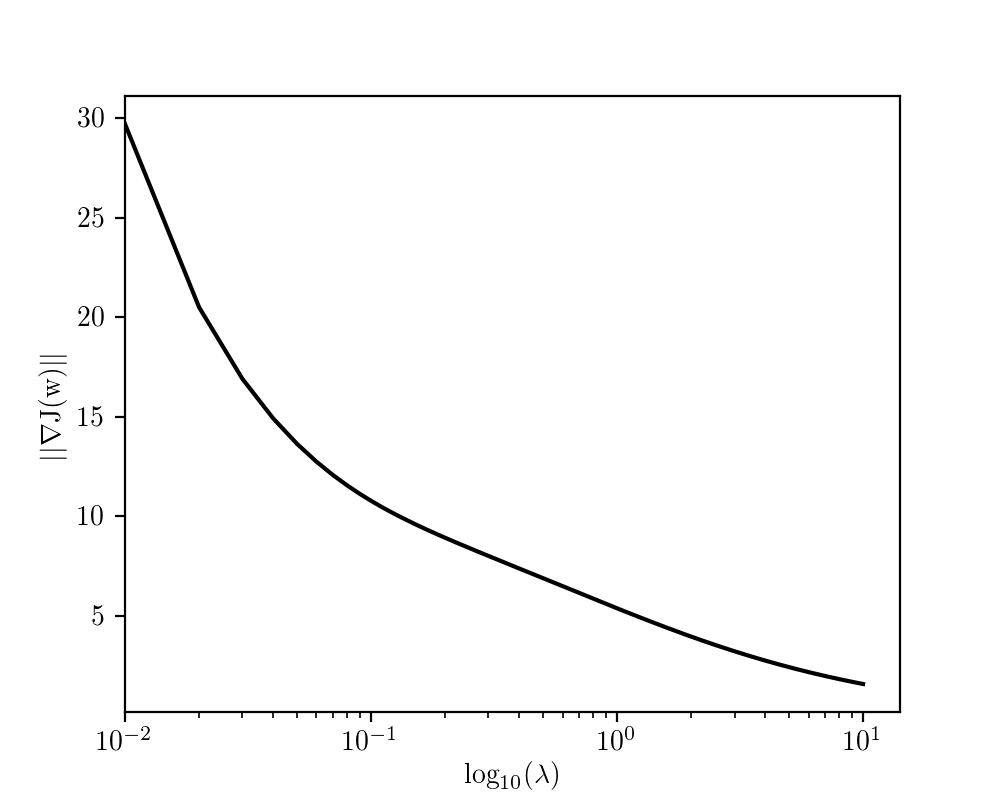
\includegraphics[width=\textwidth]{norm_lambda.png}
\caption{The effect of different $\lambda$ values on the norm of the gradient.}
\end{figure}

\begin{figure}[htp]
\centering
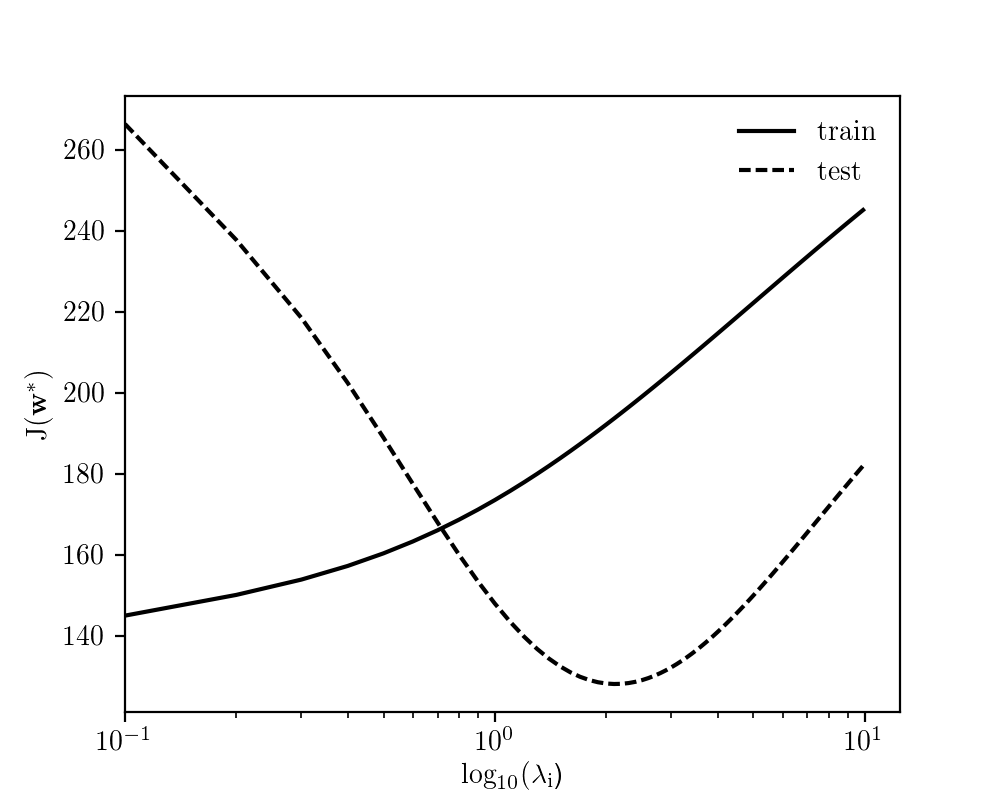
\includegraphics[width=\textwidth]{test_lambda.png}
\caption{The effect of different $\lambda$ values on the training SSE (solid) and the test SSE (dashed)}
\end{figure}

\section{10-fold cross-validation (30 pts)}

\end{document}
